%============================================================
% BAB 3 — DESAIN SISTEM
%============================================================
\chapter{DESAIN SISTEM}

Uraian pada bab ini meliputi model yang digunakan, rancangan proyek akhir, variabel
dalam proyek akhir, teknik pengumpulan data, dan analisis data. Awali pembahasan pada
bab ini dengan penjelasan umum tentang solusi yang ditawarkan untuk menjawab
\textit{Problem}.

\section{DESKRIPSI SOLUSI}

Deskripsikan solusi yang ditawarkan pada buku proyek akhir dengan jelas dan detail.
Tuliskan secara argumentatif apa saja fitur-fitur yang ditawarkan sebagai solusi baru.
Terangkan secara argumentatif tentang fitur-fitur unik pemodelan yang ditawarkan
sehingga dapat digunakan untuk menyelesaikan permasalahan.

\section{PERANCANGAN SISTEM}

Desain sistem adalah penjelasan teknikal dari solusi yang berisi urutan-urutan proses
yang akan dilakukan untuk menyelesaikan masalah. Akan lebih mudah dicerna apabila
penjelasan ini disertai dengan diagram sistem secara \textit{high-level view} sehingga
pembaca mendapatkan gambaran menyeluruh tentang desain sistem. Gambar~\ref{fig:desain_sistem}
menunjukkan bagan desain sistem yang mempunyai tiga bagian.

% ── Contoh gambar desain sistem ──────────────────────────────
\begin{figure}[H]
  \centering
  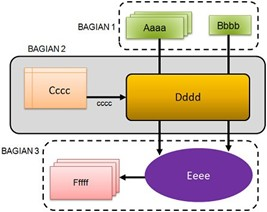
\includegraphics[width=0.6\textwidth]{gambar_desain_sistem.jpeg}
  \caption{Desain sistem dari solusi yang ditawarkan}
  \label{fig:desain_sistem}
\end{figure}

% ── Contoh gambar dengan sumber kutipan ──────────────────────
% Sumber dicantumkan di bawah gambar, di atas caption, ukuran 11pt
\begin{figure}[H]
  \centering
  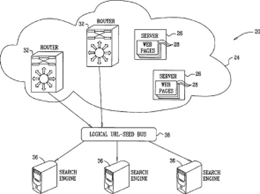
\includegraphics[width=0.6\textwidth]{gambar_kutipan.png}

  \vspace{4pt}
  {\fontsize{12}{15}\selectfont\itshape Sumber: http://alamat-sumber.com/gambar.jpg\par}

  \caption{Contoh gambar kutipan}
  \label{fig:gambar_kutipan}
\end{figure}

\subsection{Bagian 1}

Disini penulis dapat menjelaskan lebih terperinci apa saja yang ada pada bagian
ini. Jika bagian ini mempunyai sub bagian yang perlu diperjelas dalam
pembahasan, penulis dapat menuliskannya dalam sub pembahasan pada bagian ini.

\subsubsection{Aaaa}

Disini penulis dapat membahas sub bagian Aaaa lebih terperinci. Deskripsi
pembahasan seharusnya singkat, padat dan jelas, sehingga membuat pembaca
memahami maksud penulis yang tertuang dalam tulisan. Apabila pembahasan penulis
memerlukan penulisan persamaan matematis, penulis dapat menuliskannya seperti
pada Persamaan~\ref{eq:binomial}.

\begin{equation}
  (x+a)^n = \sum_{k=0}^{n} \binom{n}{k} x^k a^{n-k}
  \label{eq:binomial}
\end{equation}

Persamaan~\ref{eq:binomial} menunjukkan teorema binomial yang merupakan dasar dari
metode yang digunakan.

% ── Contoh tabel dengan sumber kutipan (tabularray) ──────────
\begin{table}[H]
  \centering
  \caption{Contoh penulisan tabel otomatis}
  \label{tab:contoh1}
  \begin{tblr}{colspec={c c c}}
    Kolom 1  & Kolom 2  & Kolom 3  \\
    Data 1-1 & Data 1-2 & Data 1-3 \\
    Data 2-1 & Data 2-2 & Data 2-3 \\
  \end{tblr}

  \vspace{4pt}
  {\fontsize{12}{15}\selectfont Sumber: Badan Pusat Pengolahan Data, 2026 \cite{buku_contoh}\par}
\end{table}

\subsection{Bagian 2}

Disini penulis dapat menjelaskan lebih terperinci apa saja yang ada pada Bagian 2 ini.
Deskripsi pembahasan seharusnya singkat, padat, dan jelas sehingga membuat pembaca
memahami maksud penulis yang tertuang dalam tulisan.

% ── Contoh tabel biasa tanpa sumber (tabularray) ─────────────
\begin{table}[H]
  \centering
  \caption{Contoh penulisan tabel 2}
  \label{tab:contoh2}
  \begin{tblr}{colspec={c c c c}}
    Kolom 1 & Kolom 2 & Kolom 3 & Kolom 4 \\
    Data 1-1 & Data 1-2 & Data 1-3 & Data 1-4 \\
    Data 2-1 & Data 2-2 & Data 2-3 & Data 2-4 \\
  \end{tblr}
\end{table}

\begin{equation}
  F = m \cdot a
  \label{eq:newton}
\end{equation}

\subsection{Bagian 3}

Disini penulis dapat menjelaskan lebih terperinci apa saja yang ada pada Bagian 3 ini.
Deskripsi pembahasan seharusnya singkat, padat, dan jelas sehingga membuat pembaca
memahami maksud penulis yang tertuang dalam tulisan.

\begin{equation}
  \lim_{x \to c} f(x) = L
  \label{eq:limit}
\end{equation}